\documentclass[12pt,letterpaper]{lsuetd}
\usepackage{setspace,graphics,dsfont,verbatim,paralist,indentfirst,amsmath,amssymb}
\setlength{\topmargin}{-0.5in}
\setlength{\textheight}{9.0in}
\addtolength{\evensidemargin}{-0.50in}
\addtolength{\oddsidemargin}{-0.50in}
\addtolength{\textwidth}{1.00in}
\setlength{\parindent}{1.75em}
\setlength{\parskip}{0ex}
\setcounter{tocdepth}{2}

\makeatletter

\begin{document}
\renewcommand\@pnumwidth{1.55em}
\renewcommand\@tocrmarg{9.55em}
\renewcommand*\l@chapter{\@dottedtocline{0}{1.5em}{2.3em}}
\renewcommand*\l@figure{\@dottedtocline{1}{0em}{3.1em}}
\let\l@table\l@figure

\pagenumbering{roman}
\thispagestyle{empty}
\begin{center}
%The title page is first created.
  STRATEGIES FOR COMPUTING THE SCALAR SELF-FORCE ON A SCHWARSZCHILD BACKGROUND: A COMPARISON STUDY WITH AN FORTRAN CODE IN C++, EXTRAPOLATING TO INFINITE DISCONTINUOUS GALERKIN ORDER, AND EXTRAPOLATING TO INFINITE SPHERICAL HARMONIC MODES

\vfill
\doublespacing
A Thesis/Dissertation \\
\singlespacing
Submitted to the Graduate Faculty of the \\
Louisiana State University and \\
Agricultural and Mechanical College \\
in partial fulfillment of the \\
requirements for the degree of \\
Master of Science\\
\doublespacing
in \\
                                       
Physics\\
\singlespacing
\vfill

by \\
Steven (Susan) Dorsher \\
B.S., Massachusetts Institute of Technology, 2004  \\
M.S., The Ohio State University, 2006  \\
M.S., University of Minnesota, 2013  \\
%If necessary, copy and paste the previous line here to include a master's degree.
December, 2017
\end{center}
\pagebreak
%The Copyright Page and Dedication sections can be added here, if desired.

%\chapter*{Copyright Page}
%\doublespacing
%\vspace{0.55ex}
%Insert the appropriate text for the copyright page here.
%\addcontentsline{toc}{chapter}{\hspace{-1.5em} {COPYRIGHT PAGE} \vspace{12pt}}
%\pagebreak

%\chapter*{Dedication}
%\doublespacing
%\vspace{0.55ex}
%Insert the appropriate text for the dedication or epigraph page here.  This part of the ETD must not exceed one page.
%\addcontentsline{toc}{chapter}{\hspace{-1.5em} {DEDICATION} \vspace{12pt}}
%\pagebreak

\chapter*{Acknowledgments}
\doublespacing
\vspace{0.55ex}
I would like to thank Peter Diener and Frank L\"{o}ffler for their guidance. Peter Diener especially has been very important to me, both as an advisor and personally. I would also like to thank Gabriela Gonzalez for the excellent opportunity to work on LIGO during the time of three detections, which provided me the funding I needed to continue the work detailed in this document. I would like to thank Juana Moreno for the opportunity to work as outreach coordinator to the LA-SIGMA Research Experience for Undergraduates program my first summer at LSU, which also helped provide funding for this research. My parents, Paul and Joanne Dorsher, also deserve a mention, both for extraordinary moral support and for the financial support they provided that helped make this possible. I would also like to thank my sister Patricia Dorsher, my grandmother Evie Dorsher and her sister Gwen Helbling, and my Aunt Peggy Bennett, and my Aunt Elaine Shirley for being my anchor. I would like to thank my friends Christy Paulson, Hope Ring, Steve Brandt, Brad Schaefer, Luke, and Josh McKeown for their company and kindness during this process. My family, friends, and loved ones are the purpose behind this work. 

%The code below adds the Acknowledgments section to the Table of Contents.
\addcontentsline{toc}{chapter}{\hspace{-1.5em} {ACKNOWLEDGMENTS} \vspace{12pt}}
\pagebreak
%The Preface section can now be added, if desired.

%\chapter*{Preface}
%\doublespacing
%\vspace{0.55ex}
%Insert the appropriate text for the preface here.
%\addcontentsline{toc}{chapter}{\hspace{-1.5em} {PREFACE} \vspace{12pt}}
%\pagebreak

\singlespacing
\tableofcontents
\pagebreak

%The code below generates the List of Tables and adds it to the Table of Contents.
\renewcommand\@pnumwidth{1.55em}
\renewcommand\@tocrmarg{8.55em}
\addcontentsline{toc}{chapter}{\hspace{-1.5em} LIST OF TABLES \vspace{12pt}}
\listoftables
\pagebreak
%The code below generates the List of Figures and adds it to the Table of Contents.
\addcontentsline{toc}{chapter}{\hspace{-1.5em} LIST OF FIGURES \vspace{12pt}}
\listoffigures
\pagebreak
%The List of Nomenclature may be included here, if desired.

%\chapter*{List of Nomenclature}
%\doublespacing
%\vspace{0.55ex}
%Provide the definitions of the symbols used in your thesis or dissertation here.
%\addcontentsline{toc}{chapter}{\hspace{-1.5em} LIST OF NOMENCLATURE \vspace{12pt}}
%\pagebreak

%The code below adds the Abstract and places it within the Table of Contents.
\renewenvironment{abstract}{{\hspace{-2.2em} \huge \textbf{\abstractname}} \par}{\pagebreak}
\addcontentsline{toc}{chapter}{\hspace{-1.5em} ABSTRACT}
\begin{abstract}
\vspace{0.55ex}
\doublespacing
Insert the text of your abstract here.  Make sure there is one blank line between the end of the Abstract text and the ``end'' command below to maintain double--spaced lines.

\end{abstract}

\pagenumbering{arabic}
\addtocontents{toc}{\vspace{12pt} \hspace{-1.8em} CHAPTER \vspace{-1em}}
\singlespacing
\setlength{\textfloatsep}{12pt plus 2pt minus 2pt}
\setlength{\intextsep}{6pt plus 2pt minus 2pt}
\chapter{Introduction}
\doublespacing
\section{Gravitational Waves}

On February 11, 2016, the LIGO Scientific Collaboration announced the
first detection of gravitational waves from a black hole binary
inspirals, occurring on September 14, 2015, with pre-merger masses of
36 $M_\odot$ and 29 $M_\odot$ and a post merger mass of 62 $M_\odot$
at a redshift of $z=0.09$~\cite{GW150914}. Two subsequent detections
followed, on December 26, 2015~\cite{GW151226} and on January 4,
2017~\cite{GW170104}, with masses that are about the same to within an order of magnitude. This detection was well-anticipated. Russel Hulse and Joseph Taylor were awarded the Nobel Prize in 1993 for their 1974 discovery of a binary pulsar. This, and similar pulsars yielded precise timing measurements of orbital period changes that corresponded to rates expected due to gravitational wave emission~\cite{hulsetaylor}. Stellar mass black holes have been known observationally for some time since the discovery of the x-ray source Cygnus X-1 in the 1960's. Active galactic nuclei at the center of galaxies have been identified as supermassive black holes since the 1960's as well. Saggitarius $A^*$, a supermassive black hole at the center of the Milky Way, was originally identified through radio astronomy and is also observable in the X-ray~\cite{sagastarmultiwavelength}, but its black hole nature has been confirmed most precisely through a 16 year study of the orbits of neighboring stars~\cite{sagastarorbits}. 

All known stellar mass black holes from x-ray sources are spinning~\cite{Bambi2017}, the LIGO gravitational wave detections suggested or were consistent with spinning black holes~\cite{GW150914}~\cite{GW151226}~\cite{GW170104}, and theoretical expectations are that angular moment from the black hole formation process should be deposited in the newly formed black hole, leaving it spinning, for the case of stellar mass black holes. For the case of supermassive black holes, there are multiple formation scenarios. One model suggests that they form from mergers of massive mass black holes from the deaths of Population I stars. Another model suggests that they are formed from large scale structure collapsing first along one dimension, then subsequently along the other two, followed by mergers into larger black holes. The third model suggests a mechanism involving initial black hole seeds at scales between these two, formed from collapsing ``clouds'' in the galactic disk. All of these models impart some spin to the initial seed black hole, that may or may not be retained in subsequent mergers~\cite{formationsmbh}. For the purposes of this document, I consider black holes without spin, using the Schwarzschild metric.


\section{Extreme Mass Ratio Inspirals}
In an extreme mass ratio inspiral (EMRI), a stellar mass black hole, or other compact object such as a white dwarf or neutron star, orbits around a supermassive black hole. It emits energy due to gravitational waves and its orbital frequency gradually increases while its orbital radius gradually decreases. Eventually it crosses the innermost stable circular orbit and, assuming it is on a roughly circular orbit, it plunges into the black hole without completing any further orbits.

The stellar mass black hole can be a factor of $10^5$ to $10^6$ smaller than the mass of the supermassive black hole in an EMRI. In an intermediate mass ratio inspiral (IMRI), the mass ratio is more like $10^2$ to $10^4$. LISA will be sensitive to EMRI's and some IMRI's. LIGO may be sensitive to some IRMI's. It is our goal to enable to the LISA community to provide gravitational wave templates to the LISA searches in time for the LISA launch in the early 2030's. Extraordinary precision is required to perform these searches, requiring an error in the period of no more $\delta P/P<10^{-6}$~\cite{LISA02062017}. This is especially challenging given that the EMRI system must be evolved over a much longer timescale than a single period due to the dependence of the particle's current position on its entire history. The timescale that suffices to make the neglect of this effect small will be much longer than a single period for any physical system. Based on dimensional considerations, this timescale scales as $M/\mu$, where $M$ is the central black hole mass and $\mu$ is the mass ratio. For a mass ratio of $10^5$, approximately $10^5$ wave-cycles must be evolved~\cite{LISA02062017}.

\section{Self force}

Consider a classical model of the atom. This is more like the Bohr model than the plum pudding model, but it doesn't make any attempt at quantization. A negatively charged electron is orbiting a positively charged nucleus. That electron emits radiation and loses energy, becoming more tightly bound. The force that causes it to move inward is called the self-force, because it is the force of the particle interacting with its own electric field ~\cite{dirac1938}.

The self-force also exists in general relativity. In the simplest possible picture of general relativity, a test particle experiencing no force moves on a geodesic. However, once we bring into our picture a compact object such as a neutron star or black hole-- which clearly has its own local curvature-- it generates a back-reaction. It is possible to obtain the self-force in general relativity from either perturbations of the metric~\cite{pound2ndOrderSelfForce} or perturbations of the particle's world-line~\cite{WardellSelfForceReview}. Either way, the small parameter governing the expansion is the mass ratio of the system. Again, the self-force is due to the interaction of the small black hole with the gravitational field itself.

In this document, we consider a slightly simpler problem, that of a scalar field on a curved space-time background. In this case, the self-force is due to the interaction of the scalar field with the particle itself. The stellar mass black hole is now a scalar delta function source that evolves along an orbit through space-time. As in the other two cases, the source causes scalar waves to be emitted that travel in all spatial directions away from the source, both toward light-like infinity and into the supermassive black hole horizon. The back-reaction causes a self-force that propels the particle slightly inward with each orbit as it loses energy to these outgoing waves. Ultimately, if evolved for that long, the particle should enter the horizon of the large black hole and then, it is beyond the scope of present day physics to say what should happen to it. 



\section{The gravitational wave sky}
Currently, there are four distinct windows on the gravitational wave universe planned or in progress. The Laser Interferometer Gravitational Wave Observatory, LIGO, probably deserves first listing, due to their recent success. LIGO observes gravitational waves using a ground based Michelson-Morley interferometer with two 4 kilometer long Fabry-Perot cavity arms. It detects strains as small as $10^{-23} Hz^{-1/2}$~\cite{LIGOsensitivity}. It has thus-far had three detections of black hole binary pairs in the tens of solar mass range. These mergers have been tracked through inspiral and merger~\cite{GW150914}~\cite{GW151226}~\cite{GW170104}, and ringdown~\cite{LIGO1e}, to produce exact tests of general relativity. LIGO has even been able to set limits on non-General Relativistic behavior, such as the magnitude of the dispersion of the intergalactic medium to gravitational waves~\cite{GW170104} and deviation of the post Newtonian parameters from those predicted from GR~\cite{LIGO1e}. The LIGO-Virgo collaboration continues searches for neutron star binary inspirals, which may have electromagnetic counterparts in the form of supernovae; pulsars, which are thought to have raised ``mountains'' on their surface causing a changing quadrapole moment-- these will also have electromagnetic counterparts; gravitational wave bursts correlated with EM, neutrino, or particle sources such as a gamma ray burst; or the cosmic or galactic white dwarf binary stochastic background radiation. In the future, KAGRA, an observatory in Japan, and IndIGO, an observatory in India, will join the search for gravitational waves, refining the collaboration's ability to locate a source on the sky. 


The cosmic microwave background (CMB) can also be used to constrain the primordial stochastic background of gravitational waves. It is a very low frequency source, with wavelengths related to the size of the observable universe ($f\sim 10^{-17} Hz$). Searches depend upon separating the polarization into two components: the B-modes, which have curl, and the E-modes, which don't. If the B-modes and the E-modes are roughly even, then tensor components of the density perturbation dominate, and gravitational waves may be present. Micro-lensing and dust are significant noise sources that must be carefully subtracted. Current searches include BICEP2, Planck, and the Keck Array. 


Pulsar timing uses the extremely precise timing of pulsars, taking their spin down into account and correlating with pairs of other pulsars. In this timing, they are looking for residual signals that may be due to supermassive black hole binaries, cosmic string cusps, and the cosmic stochastic gravitational wave background. Existing pulsar timing arrays include the Parkes Pulsar Timing Array (PPTA), the European Pulsar Timing Array (EPTA), and the North American Nanohertz Observatory for Gravitational Waves (NANOGrav). They have formed a collaboration called the International Pulsar Timing Array (IPTA). The IPTA is sensitive from $10^{-9}$ to $5\times10^{-8}$ Hz with strains on the order of $10^{-14}$ to $10^{-15}$~\cite{hobbs_dai}.



Extreme mass ratio black hole binaries are likely to be detected only by LISA. The Laser Interferometer Space Observatory (LISA) is a space-based observatory. Like LIGO, it will use interferometry to detect gravitational waves; however, it will have three arms arranged in a triangle separated by 2.5 million kilometers. Each end mirror will be in free-fall on a satellite, with the satellite stabilized by micro-thrusters. LISA Pathfinder was launched in 2015 and demonstrated the optics essential to this space-based mission can operate successfully remotely. As of June of 2017, LISA is fully funded by the European Space Agency, with NASA as a lesser partner. The launch date is set in the early 2030's. In addition to EMRI's, LISA may detect IMRI's, supermassive black hole binaries, and the primordial stochastic gravitational wave background.~\cite{LISAscienceMarch28_2017},~\cite{LISA02062017},~\cite{ELISAz}


\section{Notation}
In this manuscript, I use natural units where $G=c=1$, where $G=6.67408\times 10^{-11} m^3kg^{-1}s^{-2}$ is the gravitational constant and $c=299792458 m/s$ is the speed of light. All other quantities can be written in terms of the black hole mass. For example, lengths are naturally represented in terms of the Schwarzchild radius, $2M$, but the unit is the mass, $M$. The unit for time is also mass because the speed of light has units of length divided by time, which is one. Other units can be derived in a similar manner. Most interestingly, the units for energy are masses because, dimensionally, $E=\sqrt{M^2c^4+(pc)^2}$, in special relativity. 

I use Einstein summation notation for tensors, where a repeated Greek index implies a summation over that repeated index. For example, an $n$ dimensional tensor field of rank (1,2) transforms, in general, according to the rule
\begin{equation}
  T^\alpha_{\beta\gamma}(\bar{x}^1,\ldots,\bar{x}^n)=\Lambda^\alpha_\delta\Lambda^\epsilon_\beta\Lambda^\zeta_\gamma T^\delta_{\epsilon\zeta}(x^1,\ldots,x^n)
\end{equation}
where $\Lambda$ is the Jacobian of the coordinate transformation from $x$ to $\bar{x}$. 

Indices are raised by use of the inverse metric and lowered by use of the metric. The metric transforms contravariant one-forms, which constitute the basis, to covariant vectors, which constitute the coordinates, e.g. $u^\beta=g^{\alpha\beta}u_\beta$, where $g^{\alpha\beta}$ is the metric. However, the metric and its inverse can also be used to raise and lower indices of tensors of higher and mixed rank. The metric describes the relative distance between two coordinates on a manifold, in all $n$ dimensions, in an $n\times n$ matrix. Two sign conventions are allowed, depending on whether the time component is positive or negative, though the metric always has a negative determinant in four dimensions. In our sign convention, the Minkowski metric for flat space-time is given by


\[
\eta^{\mu\nu}=\eta_{\mu\nu}=
\begin{bmatrix}
  -1 & 0 & 0 & 0\\
  0 & 1 & 0 & 0\\
  0 & 0 & 1 & 0\\
  0 & 0 & 0 & 1\\
\end{bmatrix}
\]
Here the four dimensions are Cartesian, $t$, $x$, $y$, and $z$. The Schwarzschild metric for a spherically symmetric black-hole without charge or spin is given by
\[
g_{\mu\nu}=
\begin{bmatrix}
  -(1-\frac{2M}{r}) & 0 & 0 & 0\\
  0 & (1-\frac{2M}{r})^{-1} & 0 &0\\
  0 & 0 & r^2 & 0\\
  0 & 0 & 0 & r^2\sin^2\theta
\end{bmatrix}
\]
where $d\tau$ is the proper time, and coordinates are $t$ (the local time), $r$ (a radial coordinate that goes to zero at the singularity, $2M$ at the horizon, and infinity at spatial infinity), $\theta$ (the polar angle), and $\phi$ (the azimuthal angle). To obtain the inverse (raised) metric, simply invert the matrix representation.



\pagebreak
\singlespacing
\chapter{A simple numerical solution for a PDE using the Discontinuous Galerkin method}
\doublespacing
\section{Reduction to coupled first order differential equations}


The fundamental problem we wish to solve is to evolve the wave equation on Schwarzschild space-time with a source. However, to begin to address this problem, I implemented a one dimensional wave equation solver in C++ using the Discontinuous Galerkin method in flat space-time. The wave equation in flat space-time is given, in several different forms, by
\begin{eqnarray}
  \Box\psi=0\\
  \frac{\partial^2\psi}{\partial t^2}=\nabla\psi\\
  \frac{\partial^2\psi}{\partial t^2}=\frac{\partial^2 \psi}{\partial r^2}
\end{eqnarray}
where the final form is specialized to one dimension and $c=1$ in natural units. To numerically integrate this, it is necessary to reduce this second order differential equation to three coupled differential first order differential equations. There is a classical solution to this problem, which we follow. We introduce variables $\rho=\frac{\partial \psi}{\partial t}$ and $\phi = \frac{\partial\psi}{\partial r}$. With these definitions, and remembering that we want time evolution equations rather than spatial evolution equations, the three coupled equations become
\begin{eqnarray}
  \frac{\partial\psi}{\partial t} = \rho\\
  \frac{\partial\rho}{\partial t} = \frac{\partial \phi}{\partial r}\\
  \frac{\partial\phi}{\partial t} = \frac{\partial \rho}{\partial r}
\end{eqnarray}
This system of equations can be rewritten
\begin{equation}
  \frac{\partial u}{\partial t} = A\frac{\partial u}{\partial r} + Bu\nonumber\\
  \frac{\partial u}{\partial t} = RHS(u,t)
  \label{matrixdiff}
\end{equation}
where $u$ is the state vector consisting of $u=(\psi,\rho,\phi)$, and $A$ and $B$ are matrices. RHS stands for Right Hand Side. The C++ code has been implemented for wave equations of this generalized form, which encompasses wave equations on a Schwarzschild space-time.




\section{Spatial grids}
Our code solves a wave equation, which must first calculate a spatial derivative then integrate in time to solve a differential equation. For the spatial derivative part of the scheme, we make use of the Discontinuous Galerkin method to compute spatial derivatives, as a replacement for a finite difference scheme. Its has three primary benefits. One is that it naturally handles discontinuities in the evolved field, which is important to the effective source approach that we use when calculating orbits with a source in curved space-time. The second is that its accuracy scales exponentially with increasing polynomial order. 


\subsection{Finite difference schemes}
The classic solution to the spatial derivative problem is the finite difference scheme. In a one dimensional finite difference scheme, space is discretized into points on a line. The spatial derivative is calculated using a stencil of points that is symmetric about the point where one wants to know the spatial derivative, and extends $2n$ points beyond to either side, where $n$ is the order of the expansion. The spatial derivative is calculated from a weighted sum of the points included in the stencil, where some of the weights are negative. A stencil with $2n-1$ points in it, in one dimension, corresponds to an $n$th order expansion. It is possible to expand any order of derivative to any order of expansion. A first derivative, to second order accuracy, given by:
\begin{equation}
  D_r^{(2)}=\frac{1}{h}(-\frac{1}{2}f_{-1}+\frac{1}{2}f_1)
\end{equation}
Here the $f_{-1}$ and $f_1$ indicate the function evaluated at the grid point to either side of the $0$th grid point, where the derivative is evaluated. Here $h$ is the spacing between grid points. 
\begin{equation}
  D_r^{\prime (2)}=\frac{1}{h^2}(f_{-1}-2f_0+f_1)
\end{equation}

It is possible to extend these stencils to two and three dimensions. When considering parallelization using OpenMP, issues of synchronization must be considered. When parallelizing over many nodes, the spatial grid gets divided into blocks. At the ends of each block, the boundary cells need information from the neighboring cells to calculate the spatial derivative. For an order $n$ derivative, $n-1$ boundary cells are synchronized into buffer zones both to the left and to the right at each time step. In our code, this is not necessary, since we have parallelized with OpenMP, which uses shared memory within one node, across several (16) cores.

\subsection{The Discontinuous Galerkin method}
The Discontinuous Galerkin method breaks space into segments called elements. Within each element, the value of the field is represented by the sum of $n+1$ interpolating polynomials of order $n$, where $n$ is the order of the element. There are $n+1$ unevenly spaced nodes in the element, clustered toward the edges. At each node, exactly one of the interpolating polynomials takes on a value of one while the others are zero. An interpolating Lagrange polynomial has a functional form:
\begin{equation}
  \ell_i(r)=\prod_{j=1,j\ne i}^{n}\frac{r-\xi_j}{\xi_i-\xi_j}
\end{equation}
where $\xi_i$ is a location of a node and where $r$ is an arbitrary position~\cite{dghesthaven}. 


Omitting the details of the derivation of this method, which can be found in Reference~\cite{dghesthaven}, the procedure for calculating the spatial derivative in one dimension is to first calculate the Legendre polynomials. A matrix inversion is involved to calculate the derivative matrices, for which we use custom packages, the Template Numerical Toolkit and JAMA. It was discovered, upon parallelization with OpenMP, that TNT is not threadsafe. I rewrote most, but not all, of the code to avoid this issue; however, it would be better to replace TNT altogether if this code were developed further.

The Discontinuous Galerkin method helps damp error introduced by discontinuities in the field, provided they remain at element boundaries. We make use of this in our self-force calculations in the neighborhood of the particle, to be described in Chapter~\ref{ellipticalorb}. The numerical flux how information passes from one element to the next in the Discontinuous Galerkin method and is a way of accounting for the discontinuity in the flow between neighboring elements. The specific method we use for calculating the numerical flux breaks breaks the wave velocities into ingoing and outgoing components. At each element boundary, the state vector from external to the element is coupled to the ingoing velocity then added to the state vector internal to the element coupled to the outgoing velocity. The contribution from each boundary is distributed across the element according to a lift matrix. This is repeated at each time step. Discontinuties can exist at the boundaries, but not within an element. 



\section{Time evolution}

Time evolution in our code is handled by a fourth order low storage Runga Kutta method. Instead of the standard fourth order Runga Kutta method, this method takes five sub-time-steps, but only the most recent sub-time-step needs to be stored.

\begin{eqnarray}
  p^{(0)}=&u^n\nonumbuer\\
  k^{(i)}=&a_ik^{(i-1)}+\delta t RHS(p^{(i-1)},t^n+c_i\delta t)\nonumber\\
  p^{(i)}=&p^{(i-1)}+b_iK^{(i)}\nonumber\\
  u_h^{n+1}=&p^{(5)}
\end{eqnarray}
Here steps two and three are repeated for $i=1-5$, first $k$, then $p$, then increase $i$ and repeat. The coefficients $a_i$, $b_i$, and $c_i$ are given in Reference~\cite{dghesthaven}.

\section{Wave equation on flat space-time}

Using Gaussian initial conditions in $\psi$ and setting the $\rho$ initial conditions to the derivative of that Gaussian, I have produced the evolution shown in Figure~\ref{gaussWave}. The Gaussian marches to the right over a number of time steps, hits the periodic boundary conditions, and re-enters the one-dimensional space on the left, eventually returning to its original position. A similar progression can be seen in Figure~\ref{sineWave} for sinusoidal initial conditions.

\begin{figure}
  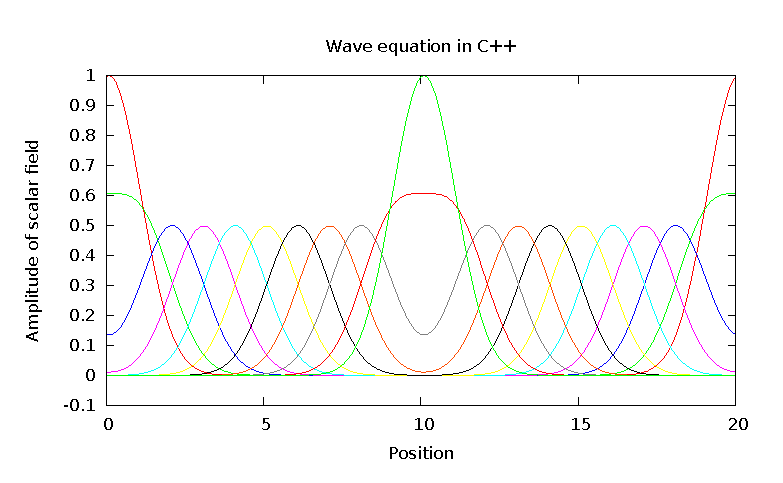
\includegraphics{gaussWave}
  \caption{Waves evolving over time for Gaussian initial conditions}
  \label{gaussWave}
\end{figure}

\begin{figure}
  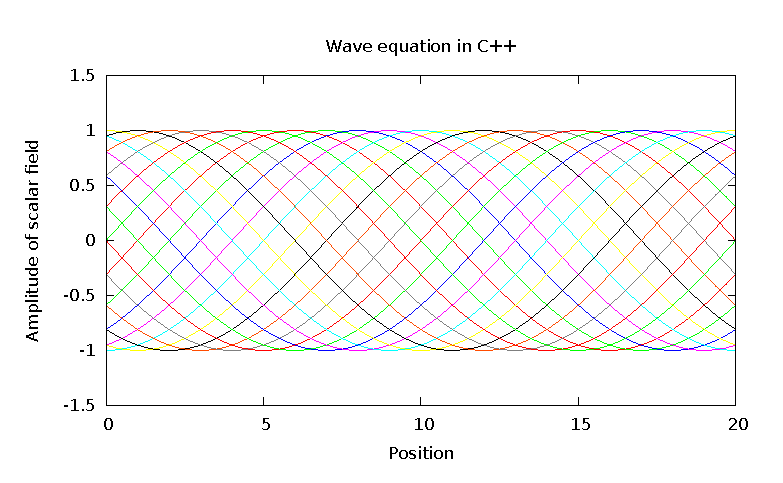
\includegraphics{sineWave}
  \caption{Waves evolving over time for sinusoidal initial conditions}
  \label{sineWave}
\end{figure}

The Discontinuous Galerkin method has truncation error that scales as $h^{n+1}$, where $h$ is the element size and $n$ is the polynomial order of the elements. The $L_2$ error is defined as the square root of the sum of the squared differences across all space, after one complete cycle of the system. The scaling of the $L_2$ error with DG order and with element size is shown in Figures~\ref{scalingorder} and~\ref{scalingelement}. The scaling matches expectations until roundoff error is hit, where the error stops improving with order or smaller element size. Not shown, this same pattern was seen for the $L_0$ error, which is the maximum error over all space.

\begin{figure}
  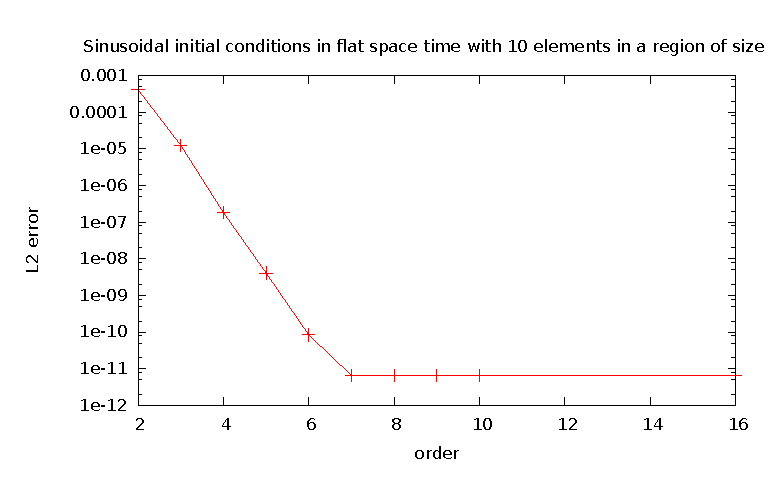
\includegraphics{sinL2WTorder}
  \caption{$L_2$ error scaling with DG order for sinusoidal initial conditions}
  \label{scalingorder}
\end{figure}

\begin{figure}
  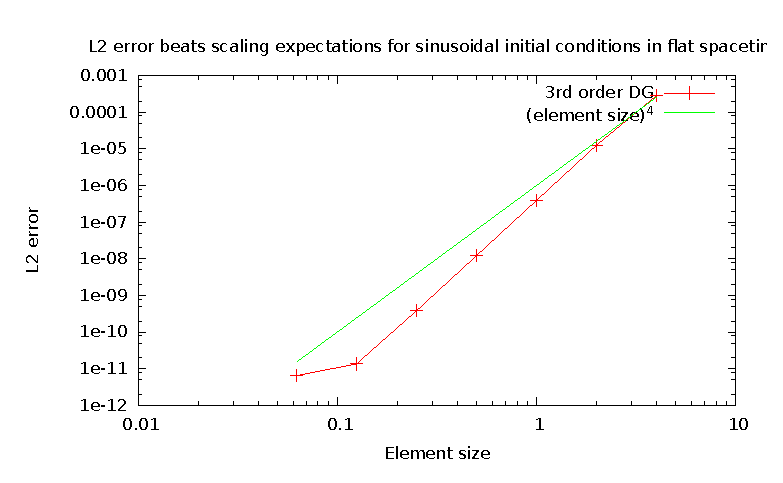
\includegraphics{sinL2WTelement}
  \caption{$L_2$ error scaling with element size for sinusoidal initial conditions}
  \label{scalingelement}
\end{figure}



\pagebreak
\singlespacing
\chapter{A scalar field on a Schwarzschild background without a source}
\doublespacing
\section{Scalar field on Schwarszchild spacetime}
Although the final goal in this field is to compute tensor waveforms that can be used as templates for LISA searches, for the purposes of obtaining the desired accuracy, it is important to improve our computational methods. We do this by performing comparison studies using scalar, rather than tensor, self force methods to make the problem more tractible. I have performed the simplest of such comparison studies-- I have reimplemented Peter Diener's Fortran scalar self-force code, with a slightly modified design, in C++. The desired goal was for the results to match to within roundoff error. This was achieved for scalar fields without a source and for scalar fields with point sources on circular orbits (see Chapter~\ref{circularorbit}.


\subsection{Scalar field wave equations}
A scalar field is a field that has one one degree of freedom at a given point in space-- rather than being a matrix, it has a single value. The scalar wave equation, on a Schwarzschild background,in the absence of a source, is, in its most abstract form, the same as in flat spacetime. 
\begin{equation}
  \Box\Psi=0
\end{equation}
The details of the implementation are a little different, to account for the curvature of space. This enters through the metric. For a scalar field, the D'Alembertian can be written
\begin{equation}
  \Box\Psi=\frac{1}{\sqrt{-g}}\partial_\mu(\sqrt{-g}\partial^\mu\Psi)=0
\end{equation}
where $g$ is the determinant of $g^{\mu\nu}$.~\cite{Wald} 

\subsubsection{Multipole moment decomposition}

\subsubsection{Tortoise coordinates}
In this code, we use a mixture of tortoise (Eddington-Finkelstein) and hyperboloidal coordinates. Tortoise coordinates have the property that they go to infinity at the horizon (scri minus) and infinity at lightlike infinity (scri plus). It is beneficial to place scri minus at an unreachable distance in coordinate space so that the boundary conditions at the horizon become trivial and there is no leakage of information from the interior of the blackhole to outside the horizon in the process of discritization. It is also beneficial to increase the number of computational elements near the horizon by compactifying the coordinates there. Tortoise coordinates transform only the radial coordinate, leaving the angular and time coordinates alone.~\cite{Wald}
\begin{eqnarray}
  t_*=t\\
  r_*=r+2GM\ln|\frac{r}{2GM}-1|\\
  \theta_*=\theta\\
  \phi_*=\phi
\end{eqnarray}
We solve the wave equation in tortoise coordinates in one region of the code. I have rederived this equation in Mathematica and verified the form that appears in Peter Diener's Fortran scalar self-force code. The wave equation in tortoise coordinates is
\begin{equation}
  \frac{d^2\psi}{dt^2}=\frac{d^2\psi}{dr_*^2}-\frac{1}{r^5}(\frac{2M}{r}+(l+1)l)(1-\frac{2M}{r})\psi
\end{equation}
$r$ is in Schwarszchild coordinates, $r_*$ is in tortoise coordinates, $l$ is the spherical harmonic l-mode (discussed below), which accounts for the angular dependence, and $\psi$ is a function of tortoise coordinates.


\subsubsection{Hyperboloidal coordinates}  
Hyperboloidal coordinates are necessary; however, because infinities are computationally unreachable. It is clear that space infinitessimally close to the horizon is important, since the curvature of space is strongest there, and it is still causally connected to the exterior region. To make the horizon reachable in a finite number of computational elements, while retaining the property that more computational elements are placed near the horizon than far away, hyperboloidal coordinates are introduced in the region closest to the horizon. In a middle region, tortoise coordinates are used. In the region furthest from the blackhole, hyperboloidal coordinates are used again to place scri plus at a finite number, yet maintaning the property that fewer computational elements are needed far away from the blackhole. Hyperboloidal coordinates are described by the transformation~\cite{hyperboloidalCoordinates}

There are a few key features. The angular coordinates are not transformed. The time coordinate preserves the stationarity of the background metric, and thus the new time variable, $\tau$, must be related to the old time variable, $t_*$, by an offset dependent only upon $r_*$, $\tau=t-h(r_*)$. For ingoing waves in the inner region, $t-r_*=\tau-\rho$ and in the outgoing region, $t+r_*=\tau+\rho$ to preserve the structure of the light cone. Bernuzzi, Nagar, and Zenginoglu define $H=\frac{dh}{dr_*}$. They introduce a compactification that depends on a window function $\Omega$~\cite{OmegaTransferFunction}, such that the tortoise radius gets redefined  $r_*=\frac{\rho}{\Omega(\rho)}$, resulting in an expression for the height function $H$ in terms of the hyperboloidal radius,  $H(\rho)=1-\frac{\Omega^2}{\Omega-\rho\Omega^\prime}$. Their final wave equation, for ingoing waves, is~\cite{hyperboloidalCoordinates}
  \begin{eqnarray}
    \partial_t^2-\partial_{r_*}^2=-(1-H^2)\partial_\tau^2\nonumber\\
    +(1-H)(-2H\partial_\tau\partial_\rho+(1-H)\partial_\rho^2-(\partial_\rho H)(\partial_\tau+\partial_\rho))
  \end{eqnarray}    
I have verified this equation, and derived the outgoing wave equation, in Mathematica.

  



\subsubsection{Initial conditions and boundary conditions}
Since there is no source for the scalar field in the C++ code, it must be set to some initial value and allowed to fall into the blackhole or radiate away its energy to infinity. A gaussian initial condition in the time derivative of the scalar field, centered at computational coordinate zero (which was some physical distance outside the black hole horizon), was chosen.   

Boundary conditions were matched automatically by the coordinate transformation between tortoise and hyperboloidal layers. At scri minus and scri plus, the boundary conditions were that the scalar field be set to zero. 



\section{Theoretical expectations}

quasinormal modes
tails

\section{Comparison of C++ code to Fortran code}
round off noise
truncation error

\begin{figure}
  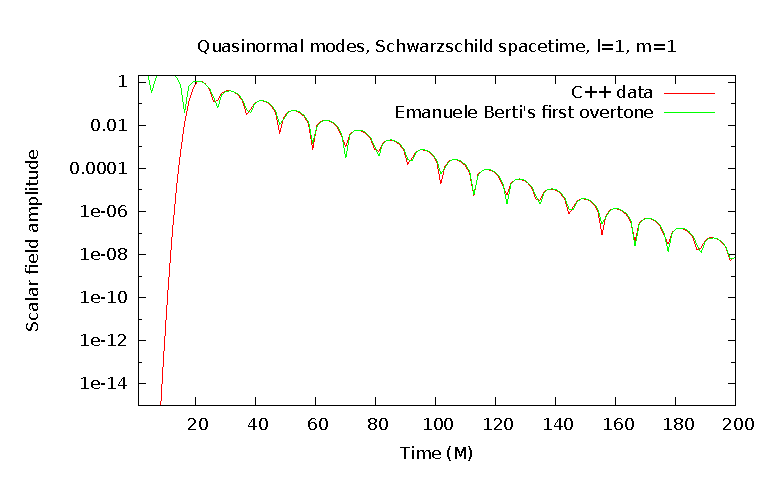
\includegraphics{l1m1qnm}
  \caption{Quasinormal mode for l=1,m=1}
  \end{figure}

\begin{figure}
  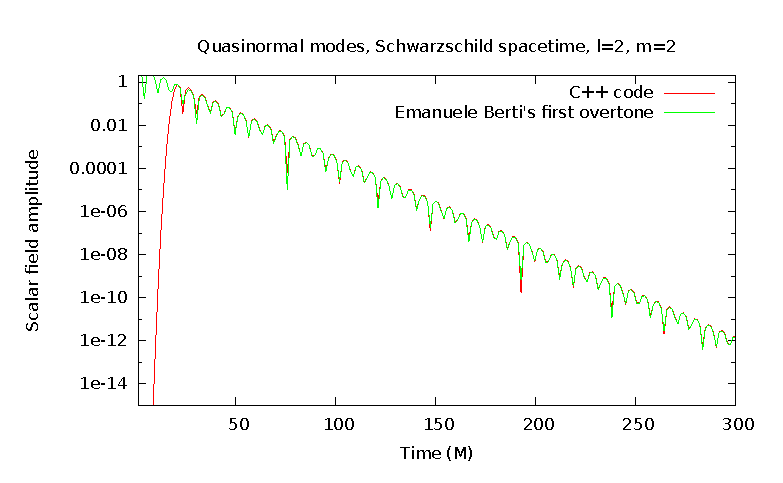
\includegraphics{l2m2qnm}
  \caption{Quasinormal mode for l=2, m=2}
\end{figure}

\begin{figure}
  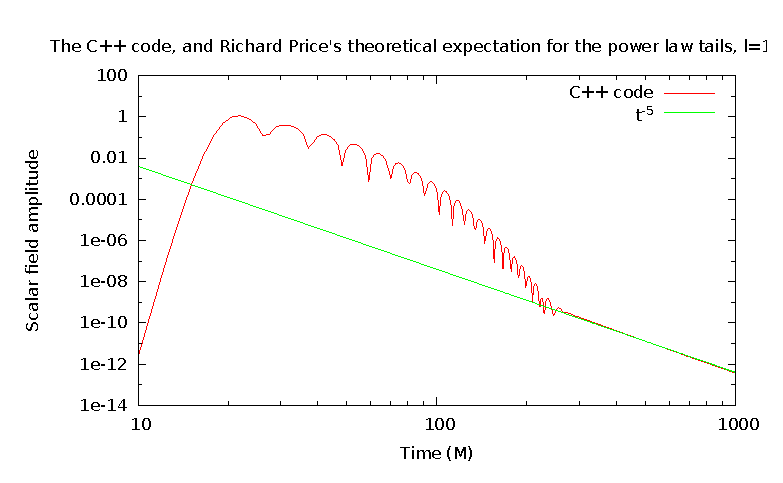
\includegraphics{l1m1tail2}
  \caption{Power law tail, l=1, m=1}
\end{figure}

\begin{figure}
  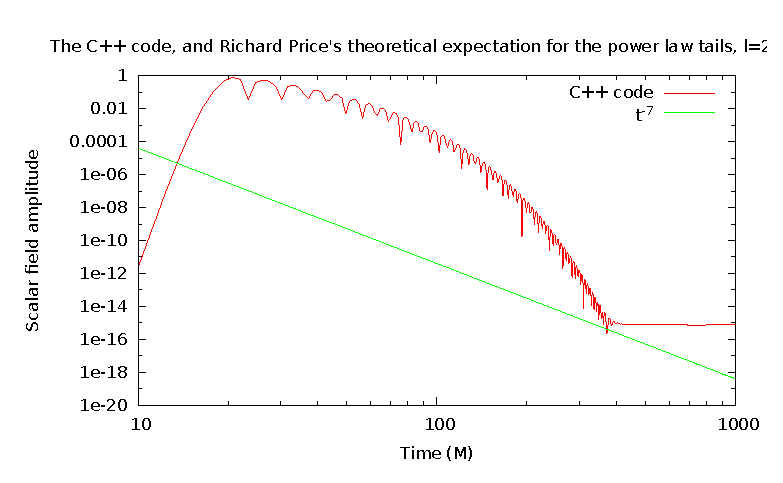
\includegraphics{l2m2tailfail2}
  \caption{Power law tail does not match expectations due to truncation error in DG method, l=2, m=2}
\end{figure}

\begin{figure}
  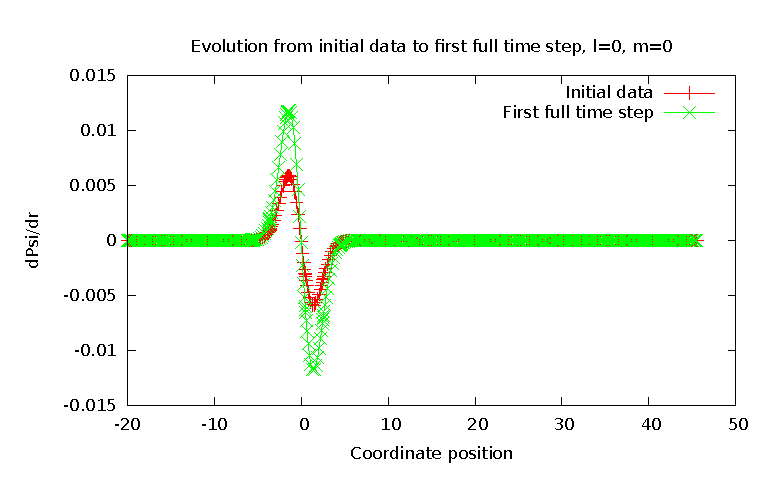
\includegraphics{phi1dl0}
  \caption{Scalar field spatial slice initial condition and first full timestep for l=0.}
\end{figure}

\begin{figure}
  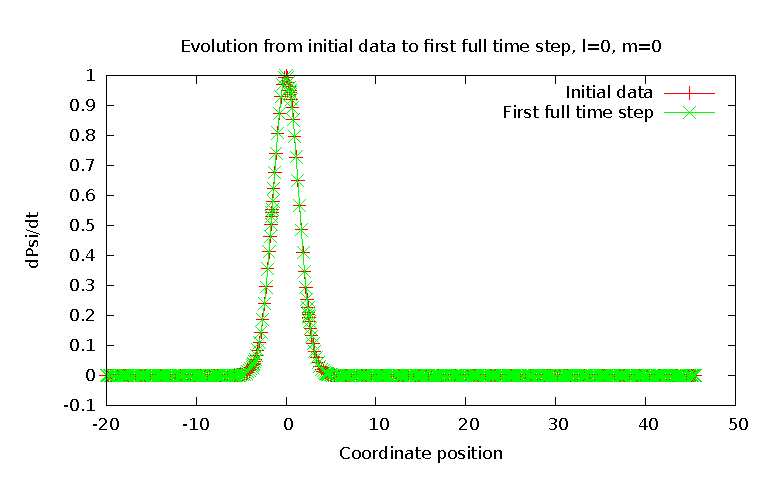
\includegraphics{rho1dl0}
  \caption{Time derivative of the scalar field spatial slice initial condition and first full timestep for l=0.}
\end{figure}

\begin{figure}
  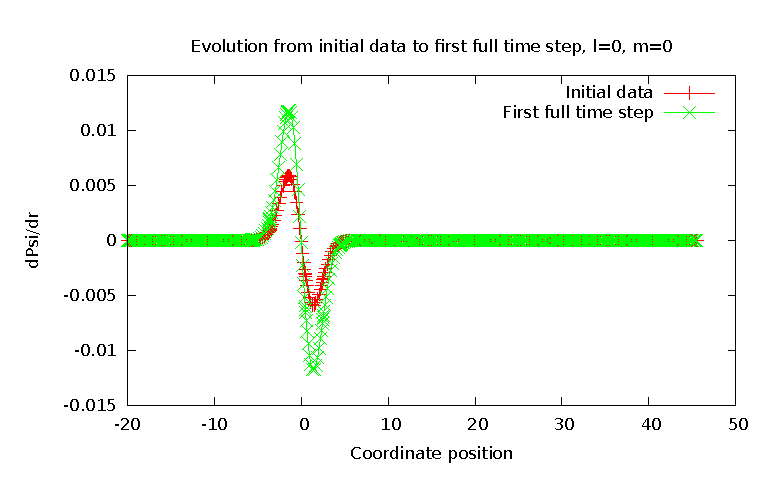
\includegraphics{phi1dl0}
  \caption{Radial derivative of the scalar field spatial slice initial condition and first full timestep for l=0.}
\end{figure}

\pagebreak
\singlespacing
\chapter{Circular orbits on a Schwarzschild spacetime}
\doublespacing
~\cite{WardellSelfForceReview}
\begin{equation}
  \Box\Psi^{ret}=-4\pi q\int\delta_4(x,z(\tau^\prime))d\tau^\prime
\end{equation}
In this equation, $\Box$ is the D'Alembertian and $z(\tau^\prime)$ is the evolving path of the source in spacetime as a function of the particle's proper time. The retarded field $\Psi^{ret}$, is defined to be the field determined by physics taking place at $t_r=t-\frac{|\vec{r}-\vec{r}^\prime|}{c}$; that is, at some distance away from the particle's path, the physical effects of gravity on the scalar field are retarded by light travel time. In the scalar approximation, the particle acts as a delta function point source, with a charge of $q$ and mass $m$. That charge may accelerate or evolve with time; see chapter~\ref{futurework}



\section{phi of t}
\subsection{Effective source}
\subsection{World tube}
\begin{figure}
\includegraphics{worldTubeItself}
\caption{Spatial slice of the world tube window function.}
\end{figure}
\begin{figure}
  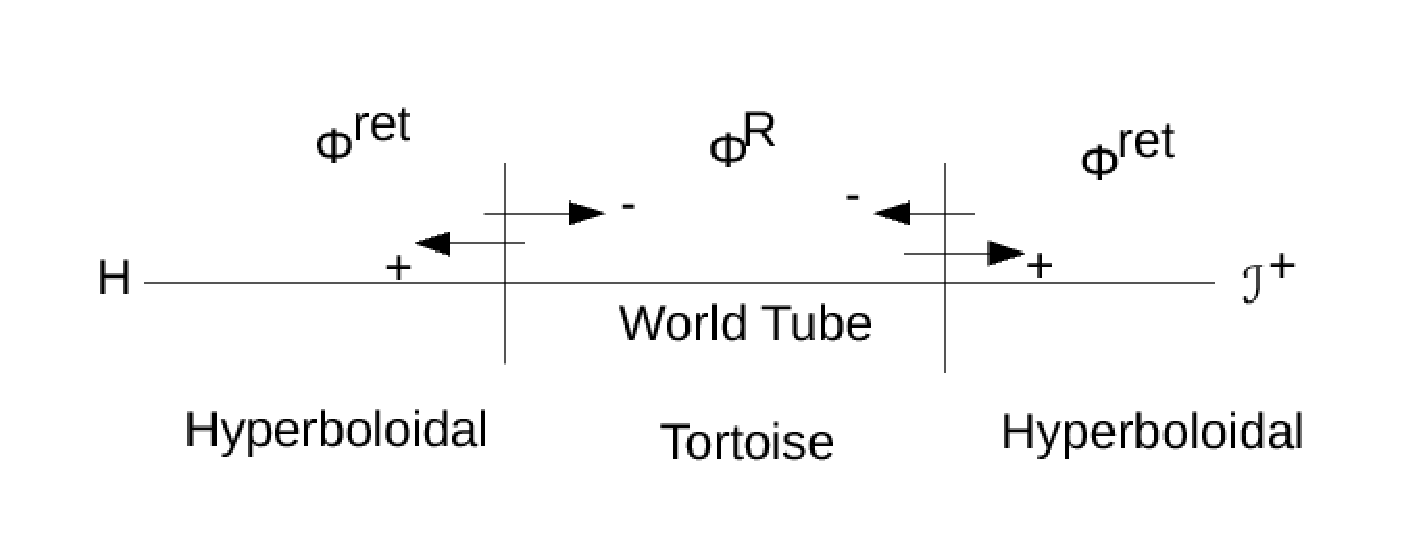
\includegraphics{WorldTube}
  \caption{Add or subtract the singular field to either side of the world tube boundary before performing the time dependent coordinate transform (or inverting it) to obtain the retarded field in the exterior region and the regularized field in the interior region.}

\end{figure}


\subsection{Comparison between C++ and Fortran codes}
\begin{figure}
  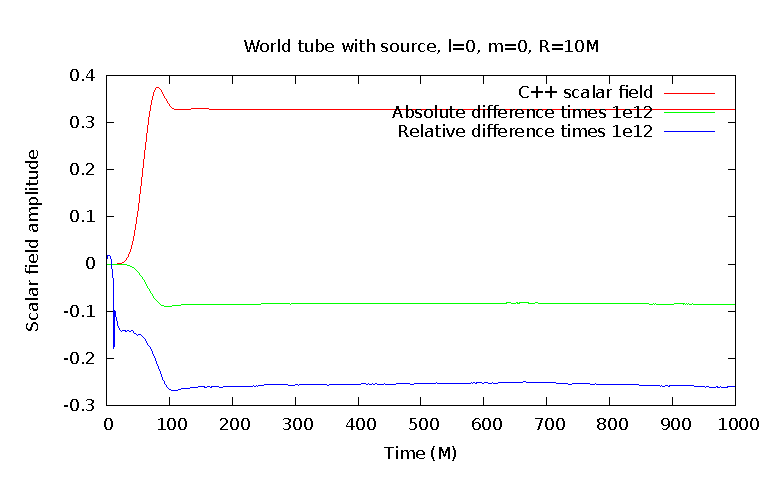
\includegraphics{wtcircl0m0}
  \caption{Comparison between Fortran and C++ codes for a particle on a circular orbit, l=0, m=0.}
\end{figure}
\begin{figure}
  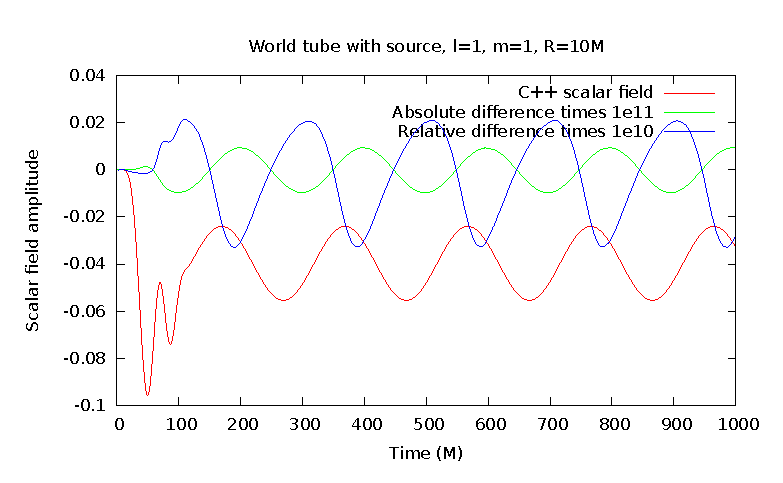
\includegraphics{wtcircl1m1}
  \caption{Comparison between Fortran and C++ codes for a particle on a circular orbit, l=1, m=1.}
\end{figure}
\begin{figure}
  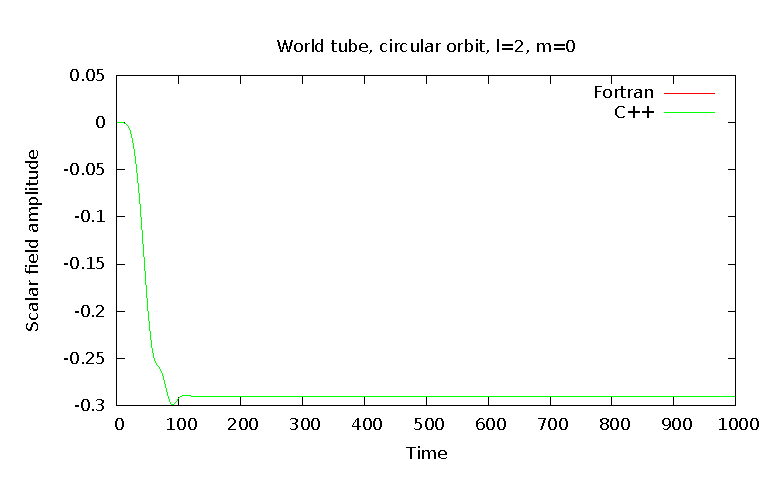
\includegraphics{wtcircl2m0}
  \caption{Comparison between Fortran and C++ codes for a particle on a circular orbit, l=2, m=0.}
\end{figure}
\begin{figure}
  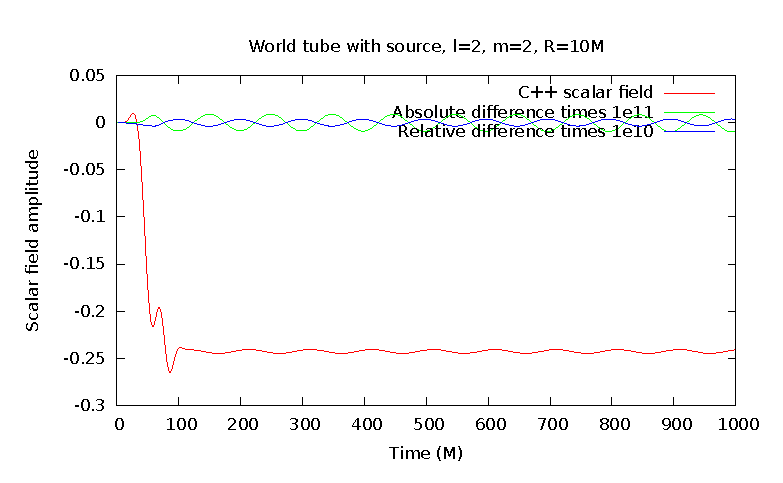
\includegraphics{wtcircl2m2}
  \caption{Comparison between Fortran and C++ codes for a particle on a circular orbit, l=2, m=2.}
\end{figure}

\pagebreak
\singlespacing
\chapter{Elliptical orbits on a Schwarzschild spacetime}
\doublespacing
\begin{figure}
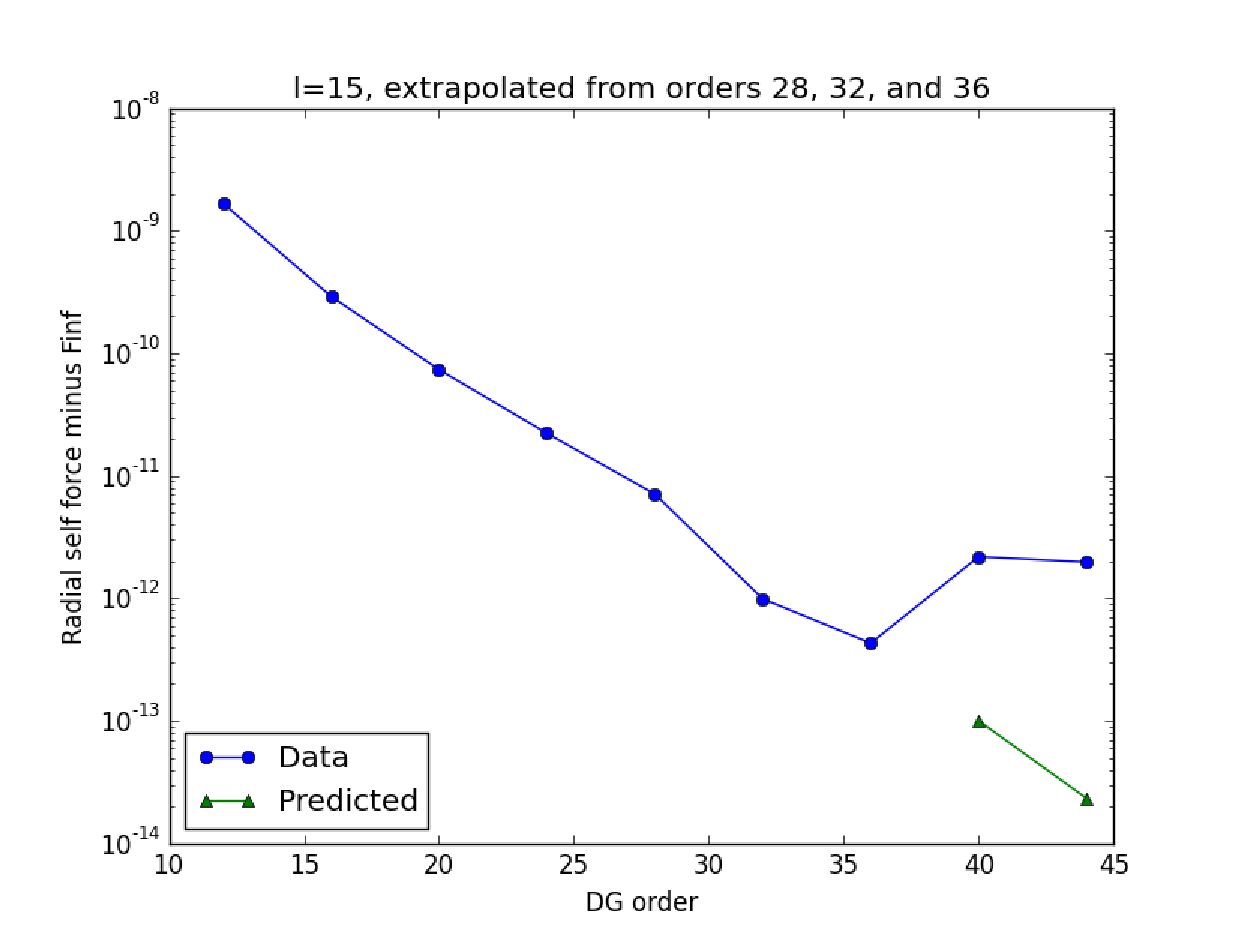
\includegraphics{/home/sdorsher/LabNotebook/20170713/extrapolate7plot}
\end{figure}

\begin{figure}
  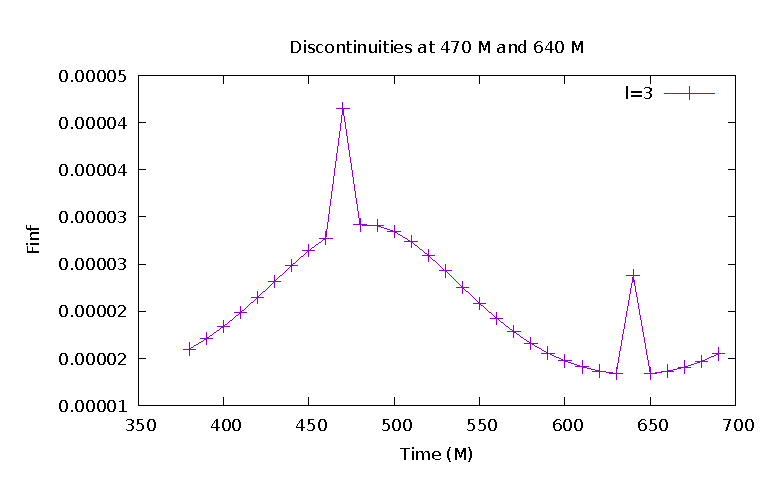
\includegraphics{/home/sdorsher/LabNotebook/20170714/finfovertimel3discontinuities}
\end{figure}




t472
\begin{table}
\begin{tabular}{ll}
Starting index & finf\\
2 & 4.18128309016e-05\\
3 & mode failed\\
4 & 4.18128307505e-05\\
5 & 4.18128308245e-05\\
6 & 4.1812830828e-05\\
\end{tabular}
\end{table}


\begin{figure}
  \includegraphics{/home/sdorsher/LabNotebook/20170719/extrapolate7t472l3i2}
\end{figure}

\begin{figure}
  \includegraphics{/home/sdorsher/LabNotebook/20170719/extrapolate7t472l2i3}
  \caption{Note that the three points used in the extrapolation are not on a line on a semilog scale-- it is not possible to fit an exponential through them. That is why this mode failed.}
\end{figure}

\begin{figure}
  \includegraphics{/home/sdorsher/LabNotebook/20170719/extrapolate7lt472l2i5}
\end{figure}

\begin{figure}
  \includegraphics{/home/sdorsher/LabNotebook/20170719/extrapolate7t472l2i6}
\end{figure}

\begin{figure}
  \includegraphics{/home/sdorsher/LabNotebook/20170719/manuallyChosenBestFinft472}
\end{figure}


\section{l=2}
\begin{table}
  \begin{tabular}{lll}
    time & starting order & finf\\
    632 & 0 & mode failed\\
    632 & 1 & 2.40975299617e-05\\
    632 & 2 & 2.40975300465e-05\\
    632 & 3 & 2.40975300114e-05\\
    632 & 4 & mode failed\\
    632 & 5 & 2.40975299291e-05\\
    632 & 6 & 2.40975299148e-05\\
    \hline
    634 & 0 & mode failed (however, 6 selected)\\
    634 & 1 & 2.39990698129e-05\\
    634 & 2 & 2.39990699318e-05\\
    634 & 3 & 2.39990698774e-05\\
    634 & 4 & mode failed\\
    634 & 5 & 2.39990697065e-05\\
    634 & 6 & 2.39990696758e-05\\
    \hline
    636 & 0 & mode failed (however, 6 selected)\\
    636 & 1 & 2.391047416e-05\\
    636 & 2 & 2.39104742806e-05\\
    636 & 3 & 2.39104742249e-05\\
    636 & 4 & 2.39104737911e-05\\
    636 & 5 & 2.39104739924e-05\\
    636 & 6 & 2.39104739079e-05\\
  \end{tabular}
\end{table}

\begin{figure}
  \includegraphics{/home/sdorsher/LabNotebook/20170720/extrapolate7t632l2i1}
\end{figure}

\begin{figure}
  \includegraphics{/home/sdorsher/LabNotebook/20170720/extrapolate7t632l2i2}
\end{figure}

\begin{figure}
  \includegraphics{/home/sdorsher/LabNotebook/20170720/extrapolate7t632l2i3}
\end{figure}

\begin{figure}
  \includegraphics{/home/sdorsher/LabNotebook/20170720/extrapolate7t632l2i5}
\end{figure}

\begin{figure}
  \includegraphics{/home/sdorsher/LabNotebook/20170720/extrapolate7t634l2i6}
\end{figure}

\begin{figure}
  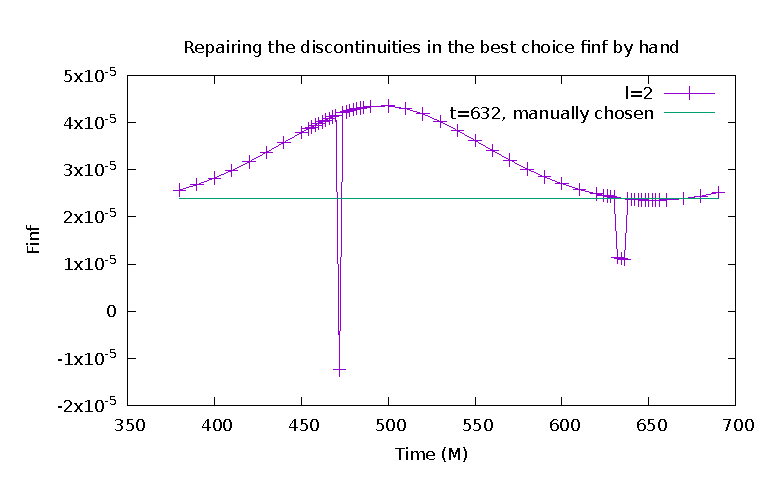
\includegraphics{/home/sdorsher/LabNotebook/20170720/bestFinfManuallyChosent632l2}
\end{figure}

\subsection{ Checking for discontinuities in $F_{\inf}$ for each each l-mode}

There are no discontinuities in $F_{\inf}$ for any of the l-modes when the median approach is used. See mode zero for an example.

\begin{figure}
  \includegraphics{/home/sdorsher/LabNotebook/20170727/finfovertimel0}
  \caption{An example of no discontinuities in $F_{\inf}$ for any of the l-modes. Mode $l=0$.}
\end{figure}


\subsection{Determining $F_{\inf}$ using maximum likelihood fits to subsegments of lines in semilog space}
Fit subsegments of lines in semilog space on DG order convergence plot after subtracting Finf for each possible starting order. pick starting order and starting and ending index of line segment with best possible chi-sq per dof (closest to one). use that finf. veto modes and starting indices that fail the alpha ratio test.

take standard deviation of surface plot as well as average.
\begin{figure}
  \includegraphics{fittingtechniqet370l0}
  \caption{l=0 mode with fit-chosen starting index produces convergence plot with nice long exponentially converging region}
\end{figure}






\label{ellipticalorb}
\pagebreak
\singlespacing
\chapter{Extrapolating the self force to infinite Disctontinuous Galerkin order}
\doublespacing
Note that it is not always possible to choose three points such that they lie on a converging exponential form, for instance, if they are not monotonic, or if they curve in the wrong direction. In these cases, I say that the ``mode failed'', and discard the result for that mode with that starting order for the extrapolation. I use extrapolation starting orders from the set 12, 16, 20, 24, 28, 32, and 36, with additional data at orders 40 and 44 that may be used as points two and three in the extrapolation. 

\begin{figure}
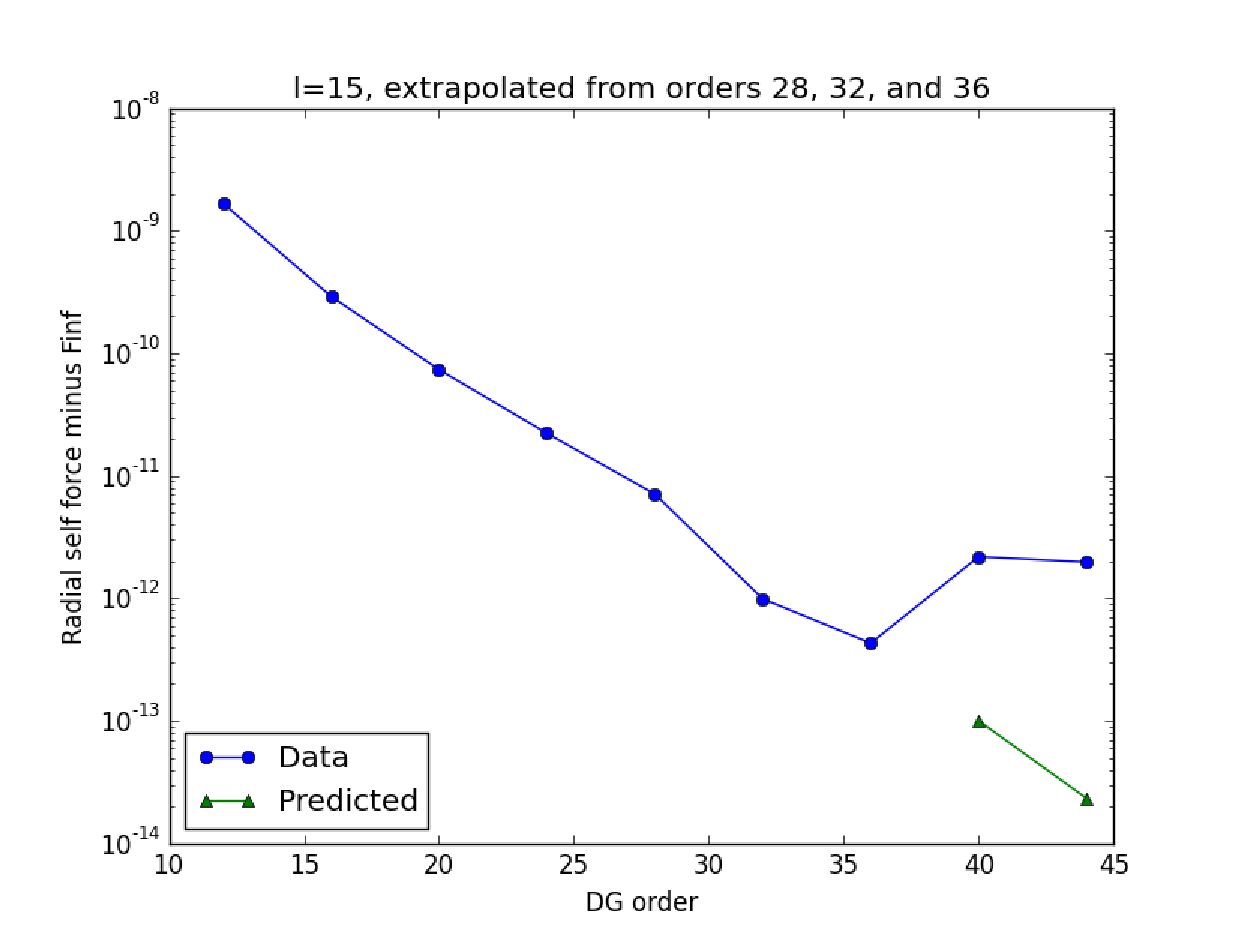
\includegraphics{/home/sdorsher/LabNotebook/20170713/extrapolate7plot}
\caption{DG convergence with order, extrapolated from highlighted points to infinite order along exponential form, which appears as a straight line in the semilog plot.}
\end{figure}



\begin{figure}
  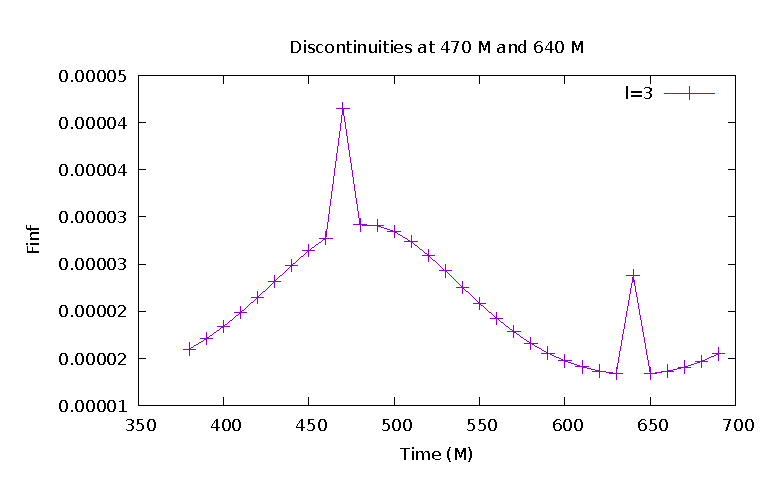
\includegraphics{/home/sdorsher/LabNotebook/20170714/finfovertimel3discontinuities}
  \caption{$F_{\inf}$ calculated in this manner, evolved over one full orbital cycle, shows some discontinuities in some l-modes.}
\end{figure}




t472
\begin{table}
\begin{tabular}{ll}
Starting index & finf\\
2 & 4.18128309016e-05\\
3 & mode failed\\
4 & 4.18128307505e-05\\
5 & 4.18128308245e-05\\
6 & 4.1812830828e-05\\
\end{tabular}
\end{table}


\begin{figure}
  \includegraphics{/home/sdorsher/LabNotebook/20170719/extrapolate7t472l3i2}
\end{figure}

\begin{figure}
  \includegraphics{/home/sdorsher/LabNotebook/20170719/extrapolate7t472l2i3}
  \caption{Note that the three points used in the extrapolation are not on a line on a semilog scale-- it is not possible to fit an exponential through them. That is why this mode failed.}
\end{figure}

\begin{figure}
  \includegraphics{/home/sdorsher/LabNotebook/20170719/extrapolate7lt472l2i5}
\end{figure}

\begin{figure}
  \includegraphics{/home/sdorsher/LabNotebook/20170719/extrapolate7t472l2i6}
\end{figure}

\begin{figure}
  \includegraphics{/home/sdorsher/LabNotebook/20170719/manuallyChosenBestFinft472}
\end{figure}


\section{l=2}
\begin{table}
  \begin{tabular}{lll}
    time & starting order & finf\\
    632 & 0 & mode failed\\
    632 & 1 & 2.40975299617e-05\\
    632 & 2 & 2.40975300465e-05\\
    632 & 3 & 2.40975300114e-05\\
    632 & 4 & mode failed\\
    632 & 5 & 2.40975299291e-05\\
    632 & 6 & 2.40975299148e-05\\
    \hline
    634 & 0 & mode failed (however, 6 selected)\\
    634 & 1 & 2.39990698129e-05\\
    634 & 2 & 2.39990699318e-05\\
    634 & 3 & 2.39990698774e-05\\
    634 & 4 & mode failed\\
    634 & 5 & 2.39990697065e-05\\
    634 & 6 & 2.39990696758e-05\\
    \hline
    636 & 0 & mode failed (however, 6 selected)\\
    636 & 1 & 2.391047416e-05\\
    636 & 2 & 2.39104742806e-05\\
    636 & 3 & 2.39104742249e-05\\
    636 & 4 & 2.39104737911e-05\\
    636 & 5 & 2.39104739924e-05\\
    636 & 6 & 2.39104739079e-05\\
  \end{tabular}
\end{table}

\begin{figure}
  \includegraphics{/home/sdorsher/LabNotebook/20170720/extrapolate7t632l2i1}
\end{figure}

\begin{figure}
  \includegraphics{/home/sdorsher/LabNotebook/20170720/extrapolate7t632l2i2}
\end{figure}

\begin{figure}
  \includegraphics{/home/sdorsher/LabNotebook/20170720/extrapolate7t632l2i3}
\end{figure}

\begin{figure}
  \includegraphics{/home/sdorsher/LabNotebook/20170720/extrapolate7t632l2i5}
\end{figure}

\begin{figure}
  \includegraphics{/home/sdorsher/LabNotebook/20170720/extrapolate7t634l2i6}
\end{figure}

\begin{figure}
  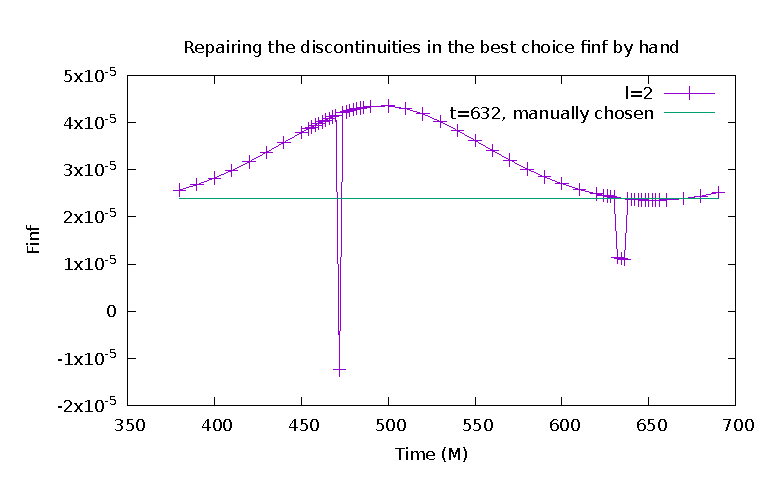
\includegraphics{/home/sdorsher/LabNotebook/20170720/bestFinfManuallyChosent632l2}
\end{figure}

\subsection{ Checking for discontinuities in $F_{\inf}$ for each each l-mode}

There are no discontinuities in $F_{\inf}$ for any of the l-modes when the median approach is used. See mode zero for an example.

\begin{figure}
  \includegraphics{/home/sdorsher/LabNotebook/20170727/finfovertimel0}
  \caption{An example of no discontinuities in $F_{\inf}$ for any of the l-modes. Mode $l=0$.}
\end{figure}


\subsection{Determining $F_{\inf}$ using maximum likelihood fits to subsegments of lines in semilog space}
Fit subsegments of lines in semilog space on DG order convergence plot after subtracting Finf for each possible starting order. pick starting order and starting and ending index of line segment with best possible chi-sq per dof (closest to one). use that finf. veto modes and starting indices that fail the alpha ratio test.

take standard deviation of surface plot as well as average.
\begin{figure}
  \includegraphics{fittingtechniqet370l0}
  \caption{l=0 mode with fit-chosen starting index produces convergence plot with nice long exponentially converging region}
\end{figure}






\pagebreak
\singlespacing
\chapter{Extrapolating the mode-summed self-force to include contributions from an infinite number of spherical harmonic modes}
\doublespacing
{\em Note that in this chapter, the optimal method for selecting $F_{inf}$ has not necessarily been used to produce all plots or all conclusions. That is a subject for later exploration and refinement.}

In the last chapter, $\psi_l$ was defined as the sum over $m$ within a specific l-mode. To obtain the total self-force, it is necessary to sum all of these l-modes, for every time, using the value of $F_{inf}$ selected for that mode. Naively, one might sum only those modes for which there is data-- only up to the maximum l-mode computed in the simulation. However, it is possible to do a fit to a functional form found in Reference~\cite{heffernan_ottewil_wardell_modesum_basisForCode} and use the analytic sum of that functional form to add the contribution from $l_{max}+1$ to infinity to the results computed from the simulation. The dependence of the m-summed self-force for a given mode on $l$, for large $l$, is shown below, modified to omit terms that are rescaled to zero by the definition of the effective source in~\cite{wardell_vega_thornburg_diener}.
\begin{eqnarray}
  F_r(l,t)=&\frac{A(t)}{(2l-1)(21+3)}+\frac{B(t)}{(2l-3)(2l-1)(2l+3)(2l+5)}\nonumber \\
  &+\frac{C(t)}{(2l-5)(2l-3)(2l-1)(2l+3)(2l+5)(2l+7)}+\ldots
  \label{lmodefitsum}
\end{eqnarray}
Here $A(t)$, $B(t)$, and $C(t)$ are constants with respect to l determined by a least squares fit. Least squares fits minimize the sum of the squared differences between the function and the data in the $y$ direction, over all values of $x_i$. For fit parameters $A$, $B$, and $C$, and $l_{max}=n-1$, the portion of the total radial self-force contributed by the l-modes extrapolated to infinity after the end of the known data is given by
\begin{eqnarray}
  \sum_n^{\infty} F_r(l) = &\frac{An}{4n^2-1}+\frac{Bn}{3(9-40n^2+16n^4)}\nonumber\\
  &\frac{Cn}{5(2n-5)(2n-3)(2n-1)(2n+1)(2n+3)(2n+5)}+\ldots
\end{eqnarray}
Although Peter Diener's Fortran code implements this sum, I have analyzed it in an independent way to establish choices of $l_{min}$ and $l_{max}$ and to establish best choice DG orders for the code. In my computations, I have terminated the ``end of the known data'' at the end of the fit region, on the theory that I am simulating having more or fewer total l-modes available to me by including more or fewer l-modes in my fit.

\section{Fitting techniques and choice of starting mode}
\label{fitting}
A good fit should not have a systematic deviation to one side of the data. Such systematic deviations are often introduced in power-law fits in experimental data because the error stays about the same as the value decreases. Thus, constant errors are used in the fit, and data with a weak signal is given less importance.

However, it is difficult to apply this expectation to data in the truncation error regime of data generated from a numerical simulation. There are two differences. One is that the error is biased. While a good fit should still pass through the middle of the data in some sense, the truncation error may result in systematic deviations of the functional form of the self-force with l-mode. We believe we have corrected this to first order using a Richardson extrapolation, but higher order deviations may remain.

Secondly, the second order error is not necessarily expected to remain constant with l-mode. Ideally one would do a second order Richardson extrapolation to take the second order error into account and compute the truncation error, but our data is too sparse in starting orders with solutions. Instead, I assume the error is random and scales in two different specified manners, $\sigma^{-1}$ and $\sigma^{-2}$. This is neither the classical manner of computing the roundoff noise nor the truncation noise; however, it should improve a least squares fit and therefore improve stability and accuracy in the simulation.  

In these fits, I minimize the classic $\chi^2$ with weights, as follows
\begin{equation}
\chi^2=\sum_i \frac{(y_i-f(x_i))^2}{\sigma_i^2}
\end{equation}
Since the $\sigma_i$ weights do not represent proper statistical uncertainties, the normalization of the weights is unimportant, unless they are used to interpret the ``goodness'' of a fit in terms of a reduced chi-squared. Since the error behaves in an unknown, possibly highly correlated, deterministic, manner, cation is warranted in doing so. I have examined weights that are constant (effectively no weight), that  scale as $l^{-2}$, and that scale as $l^{-1}$. The first is motivated by standard fitting techniques and is the default solution, while the second is motivated by the nature of the first order scaling behavior of the function to which we fit the l-modes, and the third is motivated by the desire to find something that behaves well in both the truncation error and roundoff error regimes. Figure~\ref{sigmafit} shows the functional form of the l-mode fit with three different choices of weights. Figures~\ref{8badfit} and~\ref{14goodfit} show that for all choices of weight scaling, a starting l-mode of 14 is a reasonably good fit, while significantly lower starting modes are a bad fit for three terms in the l-mode fit expansion. These figures also show that the choice of sigma can make a small difference in the goodness of the fit at high l-mode, which is important for extrapolation to infinite l-mode. However, Figure~\ref{scatterfig} shows that for a range of $l_{min}$ versus $l_{max}$, the variation in the total radial self force due to variation over start and stop range in the fit is small compared to the variation between between $l^{-2}$ scaling and constant scaling (circles and triangles). 

\begin{figure}
  \includegraphics{fiterrscalecorrect3term570l1}
  \caption{The l-mode convergence behavior and three different fits to it using three terms in the l-mode fit sum of Equation~\ref{lmodefitsum}. The three different fits represent different choices of weights in the least squares fit.}
\label{sigmafit}
\end{figure}

\begin{figure}
\includegraphics{fitresiduals3terms570l8}
\caption{Fit residuals for three different least squares weight scalings starting from $l_{min}=8$ to $l_{max}=30$. Notice that this is a bad fit, due to the strong correlated skews to either side of the axis.}
\label{8badfit}
\end{figure}

\begin{figure}
\includegraphics{fitresidulas3terms570l14}
\caption{Fit residuals for three different least squares weight scalings starting from $l_{min}=14$. This is a much better fit than $l_{min}=8$ to $l_{max}=30$ both due to the smaller correlated deviations from zero and due to the smaller amplitude of the residual.}
\label{14goodfit}
\end{figure}

\begin{figure}
  \includegraphics{3Dscatterwithwithoutsigmalminlmax}
  \caption{The difference between the triangles and the circles shows that the difference in the total radial self force between the presence of a $\sigma\sim l^{-2}$ weight and no weight is unimportant compared to the difference in the total radial self force between various start and end points of the l-mode fit.}
  \label{scatterfig}
\end{figure}

\section{Roundoff noise and choice of end mode}

In Figure~\ref{surface234big} roundoff noise is evident at higher $l_{max}$ choices, where $l_{min}$ is the minimum l-mode included in the fit and $l_{max}$ is the maximum l-mode included in the fit. This is most true of times near apastron. Note that there is not a large difference between two and three terms, and that four terms is less smooth a surface, suggesting that it is more subject to variations in the fit due to a poor fit at high l. The systematic deviations in the plot are correlated because all regions to the right of mode 27 include mode 27 in the fit, for example. The upsurge at high l is most readily attributed to roundoff noise. In Figure~\ref{surface234small}, a smaller region of $l_{min}$ versus $l_{max}$ space has been chosen to form the surface plot where roundoff noise is excluded. Three terms is preferred due to its stability within this region.

\begin{figure}
  \includegraphics{bestfinflminlmax234terms635fullrange_perihelion}
  \caption{A surface plot of $F_{inf}$ generated using the median method, t=635, 2, 3, and 4 term fits over a broad range of $l_{min}$ and $l_{max}$ values. Note the roundoff noise at high $l_{max}$ that creates an upsurge in the surface. This is at apastron, where the roundoff noise effect is strongest. 2 is blue, 3 is green, 4 is orange.}
  \label{surface234big}
\end{figure}

\begin{figure}
  \includegraphics{bestfinflminlmax234termst635smallrange_perihelion}
  \caption{A surface plot of $F_{inf}$ generated using the median method. t=635, 2, 3, and 4 term fits over a small range of $l_{min}$ and $l_{max}$. This is near apastron where the roundoff noise is a dominant effect in the larger range of $l_{max}$.  No roundoff noise is evident in this range of $l_{min}$ and $l_{max}$ so it is a suitable range to consider at all times. 2 is blue, 3 is green, 4 is orange}
  \label{surface234small}
\end{figure}



\section{Results and errors}

Figure~\ref{totalselfforcevt} shows the evolution of the total self force over time. First it has been extrapolated to obtain $F_{inf}$ using the three-point DG order exponential convergence extrapolation technique, and the optimal starting order has been chosen. Then the modes computed in the simulation have been summed numerically from $l=0$ up to some $l_{max}$, and a fit from $l_{min}$ to $l_{max}$ has been used to extrapolate the sum to infinite $l$, to obtain the total radial self-force, at each time. 


\begin{figure}
  \includegraphics{totalselfforcevt2.eps}
  \caption{This is the total radial self force calculated using a l-mode sum including a contribution directly summing $F_{inf}$ from $l=0$ to $l=25$ and a contribution obtained using an analytic sum of the three term fit in Equation~\ref{lmodefitsum}. $F_{inf}$ is measured using the asymptote method defined in Chapter~\ref{finfchap} for selecting the best starting order}
\label{totalselfforcevt2}
\end{figure}


\subsection{Relative and absolute differences}

Figure~\ref{relErrSelfForceBigSmall} shows the relative difference between the total radial self force measured in two different ways. The self-force values in each surface plot shown in Figures~\ref{surface234big} and~\ref{surface234small} were averaged to obtain better estimates of the total radial self force as a function of time. This plot shows the relative difference. I use averages and standard deviations of correlated data with biased errors of data that is not fundamentally random, so they cannot be interpreted in the strictest of statistical senses; however, they should still provide some indication of the central value and spread of the data.

The relative difference introduced by the starting and end point of the fit is on the order of $10^{-4}$ based upon these averages. If individual modes were considered rather than averages, we might expect to see the resolution decrease by a factor of the square root of the ratio of the size of the two regions being averaged, due to the central limit theorem. That's a factor of $\sqrt{7\times 6}{4\times 4}=1.6$, which is not significant on the scale of four orders of magnitude. 


\begin{figure}
  \includegraphics{relErrBigSmallRangeOverTime.eps}
  \caption{The relative difference between total self force determined by averaging large versus small ranges of total radial self-force $l_{min},l_{max}$ surfaces, as a function of time is at the $10^{-4}$ level.}
  \label{relErrSelfForceBigSmall}
\end{figure}


Figure~\ref{relErr23terms} shows the relative difference between using two and three terms in the fit to compute the total radial self force, as a function of time. Again, this is random, decreasing with time, and at the $10^{-4}$ level. 


\begin{figure}
  \includegraphics{relativeError23termSelfForce.eps}
  \caption{The relative error of the total radial self-force, comparing two to three terms in the l-mode fit.}
  \label{relErr23terms}
\end{figure}

The error due to the choice of the number of terms in the fit is comparable to the error due to the choice of start and end modes and the error due to our inability to use a first order Richardson extrapolation in real time. These errors are all at the level of a relative error of $10^{-4}$. The error due to the choice of fit method, visible from the offset between the triangles and circles, corresponding to the use of weights and no weights, can be seen in Figure~\ref{scatterfig} and is subdominant to the error introduced by the choice of $l_{min}$ and $l_{max}$ by at least an order of magnitude. 




\subsection{Fractional errors}


I obtain the fractional error, within a given method for choosing the best self force, by dividing the standard deviation of the total self-force, over a range of $l_{min}$ and $l_{max}$ by the average. This is shown for median and fit methods in Figures~\ref{medfracerr} and~\ref{fitfracerr}, respectively. The two methods are clearly not consistent in detail of their evolution, though they give roughly the same order of magnitude averaged over time. The absolute error is the standard deviation itself. The absolute error, as a function of time, compared to the self-force itself, is shown in Figure~\ref{twopeaks}. The two peaks do not obviously match periastron, apastron, or any specific phase of the orbit. {\em There is further work to be done here, specifically, I would like to redo this with the asymptote method.}


\begin{figure}
  \includegraphics{fractionalErrorSelfForceOverTime3termMedian}
  \caption{Fractional error in total radial self force, with average and standard deviation calculated over the surface shown in Figure~\ref{surface234small}. Fractional error is defined as standard deviation divided by average. This figure is for 3 terms in the fit, using the median method. Fractional error is at the level of $10^{-3}$. $F_{inf}$ was determined using the median method to determine $F_{inf}$.}
  \label{medfracerr}
\end{figure}

\begin{figure}
  \includegraphics{fractionalErrorOverTimeFits}
  \caption{Fractional error in the total radial self force, with average and standard deviation calculated over the surface shown in Figure~\ref{surface234small}. Fractional error is defined as standard deviation divided by average. This figure is for 3 terms in the fit, using the fit method to determine $F_{inf}$. Fractional error is at the level of $10^{-3}$. $F_inf$ was determined using the fit method.}
  \label{fitfracerr}
\end{figure}


\begin{figure}
  \includegraphics{structErrFitMethod}
  \caption{The structure of the standard deviation of Figure~\ref{surface234small} in comparison to the evolution in time. This is for the fit method for determining $F_{inf}$.}
  \label{twopeaks}
\end{figure}

Relative error compares one model to a different model. Fractional error compares the spread of parameters within a model. The order of magnitude larger fractional error in the l-mode start and end points than in the relative error measurement of these start and end points points to the importance of the corrections in the surface in Figure~\ref{surface234small}. To obtain an estimate of the error that is better than a two order of magnitude range from $10^{-3}$ to $10^{-4}$, it is necessary to perform either a proper second order Richardson extrapolation or a proper statistical study using covariances, hypothesis testing, and an as yet undiscovered method of handling biased estimators and unmodelled noise. 


\section{Best choice $l_{mins}$ and $l_{max}$'s and best choice DG orders}

$l_{min}$ can be as low as 14 and as high as 17, and $l_{max}$ can be as low as 22 and as high as 25 without encountering roundoff or truncation error. The errors are dominated by correlations in the choice of the start and end modes. Relative error and fractional error, in the sense of a standard deviation divided by an average, appear to measure different things when correlated measurements are involved. If we take relative error as the quantity of interest due to standards of the numerical relativity field, the dominant error is at the $10^{-4}$ level. The primary effects are the selection of the number of terms in the mode-sum and the selection of start and end modes to achieve the regime in which the fit is valid and to eliminate roundoff noise. These results are very preliminary and further investigation is intended. {\em In particular, I will need to reproduce some of these plots and re-evalute the conclusions using the asymptote method or a further developed version of the fit method.} We hope they will improve.


\pagebreak
\singlespacing
\chapter{Improving mode fits via a power law scaled weight factor in $\chi^2$ sum}
\doublespacing
\section{Plans for the more distant future}
First, I will continue to work toward a solution to the peak in the relative difference between $F_{inf}$ and the best DG order, 36, in Figure~\ref{relmixed} using the asymptote method for determining $F_{inf}$. I will also need to re-evaluate most of the conclusions of Chapter~\ref{lmode} and possibly reassess best start and stop modes for the fit. Then I will update our comparison study using Niels Warburton's geodesic code for low l-modes to higher l-modes and use more recent versions of both codes. I will report the results to Niels Warburton and Peter Diener. 

I also plan to run Peter Diener's simulation of scalar self-force on a Schwarzschild background for generic orbits including a back-reaction which causes the orbit to evolve away from a geodesic.

This is distinct from Niels Warburton's code, which uses frequency domain initial data that assumes the particle has been on the same geodesic for all time. Generating the initial data in the frequency domain gives high precision because the bandwidth of the orbit is narrow in a two dimensional frequency phase space controlled by $\phi$ and $\chi$. Because of a narrow bandwidth, finite bin sizes, and aliasing effects, it is difficult to evolve a gradual change in the orbit in the frequency domain. However, it is excellent for generating initial conditions, since the particle's past history must in principle be known for all time. 


In the time domain, the state of the field itself naturally accounts for the past history of the particle. It may be evolved using two methods, the osculating orbits approach or the geodesic evolution approach. The osculating orbits approach should have more accuracy due to the monotonic evolution of $\chi$ and $\phi$ and the slow evolution of $p$ and $e$, as opposed to the oscillating evolution of $r$ and $t$ in the geodesic approach. I will compare the osculating orbits approach with Niels Warburton's frequency domain initial conditions evolved in the time domain using the geodesic evolution approach. 


Peter Diener, Ian Vega, Barry Wardell, and Steven Detweiler~\cite{diener_vega_wardell_detwieler_2012} have previously published on self-consistent evolution of a particle around a Schwarzschild black-hole; however, it did not have sufficient accuracy. We are attempting to improve the accuracy using entirely different numerical methods.

\section{Self-consistent evolution}



The long term goal of the field is self-consistent evolution. To extend the wave equation to that produced by a particle on a self-consistent orbit, it is necessary to include several additional effects. In addition to the wave equation with a source, the orbit evolves according to the geodesic equation, via the acceleration. The particle also gains or loses mass equal to the work being done on it. 

\begin{eqnarray}
  \Box\Psi^{ret} =& -4\pi q \int\delta_4(x,z(\tau^\prime))d\tau^\prime\nonumber\\
    ma^\alpha=&q(g^{\alpha\beta}+u^\alpha u^\beta)\partial_\beta\Psi^{R}\nonumber\\
    \frac{\partial m}{\partial \tau}=&-q u^\alpha\partial_\alpha \Psi^R_\alpha
    \label{genericev}
\end{eqnarray}
The second equation gives the back-reaction due to acceleration of the particle. Here, $\Psi^R$ is the regularized field. The third equation governs the self-consistent evolution of the mass of the particle.~\cite{WardellSelfForceReview}

There are two methods for evolving the orbit that we may use, already implemented in the code by Peter Diener: geodesic evolution and osculating orbits~\cite{pound_poisson}.

\subsection{Geodesic evolution}
The geodesic equation is modified to include a force term on the right hand side in the presence of a self-force or external force~\cite{Carroll}.
\begin{equation}
  \frac{d^2x^\mu}{d\tau^2}+\Gamma^\mu_{\rho\sigma}\frac{dx^\rho}{d\tau}\frac{dx^\sigma}{d\tau}=a^\mu
\end{equation}
This equation, together with Equations~\ref{genericev}, provide the basis for the generic evolution code when the geodesic evolution method is used. 

\subsection{Osculating orbits}

An alternative approach is possible, based upon Reference~\cite{pound_poisson}. In a Schwarzschild spacetime, if the effect of the small black hole is neglected, there is a Killing vector along the time direction and along all three spatial directions, resulting in linear momentum conservation in all directions and hence angular momentum conservation. It is natural to evolve in a physical process that is closely related to these quantities. The eccentric orbit geodesic parameters $p$ and $e$ (semilatus rectum and eccentricity) are chosen (see Chapter~\ref{ellipticalorb}). In the self-consistent evolution, the orbit is accelerated from one geodesic to a neighboring geodesic, and gradually evolves through from one tangent geodesic to the next over time. In this process, $p$ and $e$ are updated via a series of ordinary differential equations with extraordinarily complicated right hand sides. This is done using the same RK4 routine that is used to solve the wave equation. It will hopefully be more accurate than the geodesic evolution scheme because angular parameters $\phi$ and $\chi$ monotonically and smoothly increase while $p$ and $e$ evolve slowly, reducing truncation error. This is in contrast to the accumulation of error introduced through oscillations in $r$ and $t$ in the geodesic method. In the self-consistent approach, the mass and acceleration will also be evolved, eventually. 



\section{Timeline}

I believe it will take me roughly one to four months to complete the re-evaluation of the methods in Chapter~\ref{lmode}. It may take substantially longer if it is necessary to obtain large amounts of data to examine the second order Richardson extrapolation or if it is necessary to use formal statistics for biased, correlated errors with hypothesis testing.

I expect that extracting physics from, and helping to debug and possibly write code for, the Warburton/Diener simulations to obtain a comparison between the geodesic and osculating orbits approaches with the frequency domain initial data will take a year. Writing it into a paper and getting it published will take another year.

That totals about two years, when some leeway is allowed for writing the thesis. 

The self-consistent evolution, in the sense of mass evolution and an accelerating source, will not be included in the thesis unless things progress a lot faster than expected. 



\label{sigmachap}
\pagebreak
\singlespacing
\chapter{Future work: generic orbits via the osculating orbits framework}
\doublespacing
\section{plans for the future}
going to test Peter Diener's generic orbits and help him develop them further.
\subsection{methods}
effective source
osculating orbits
time dependent coordinate transformation
world tube
already implemented with accelerated orbits though I have not run these.
future work: make self consistent evolution work. 

\pagebreak
\singlespacing
%To insert additional chapters, copy the previous five lines, using chapterX as the argument of the 
%\input command for Chapter X, where X=6,7,8,...
\addtocontents{toc}{\vspace{12pt}}
\addcontentsline{toc}{chapter}{\hspace{-1.6em} REFERENCES}
\begin{thebibliography}{999}
\vspace{0.9em}
\bibitem{GW150914}
LIGO Virgo Collaboration. (2016). Observation of Gravitational Waves from a Binary Black Hole Merger. {\em Phys. Rev. Lett.} 116, 061102.

\bibitem{GW151226}
LIGO Virgo Collaboration. (2016). GW151226: Observation of Gravitational Waves from a 22-Solar-Mass Binary Black Hole Coalescence. {\em Phys. Rev. Lett} 116, 241103.
  
\bibitem{GW170104}
  LIGO Virgo Collaboration. (2017). GW120104: Observation of a 50-Solar-Mass Binary Black Hole Coalescence at Redshift 0.2. {\em Phys. Rev. Lett.} 118, 221101.

\bibitem{LIGO1a}
  LIGO Virgo Collaboration. (2016). Observing Gravitational-wave Transient GW150914 with Minimal Assumptions. {\em Phys. Rev. D} 93, 122004.

\bibitem{LIGO1b}
  LIGO Virgo Collaboration. (2016). GW150914: First Results from the Search for Binary Black Hole Coalescence with Advanced LIGO. {\em Phys. Rev. D} 93, 122003.
\bibitem{LIGO1c}
  LIGO Virgo Collaboration. (2016). The Rate of Binary Black Hole Mergers Inferred from Advanced LIGO Observations Surrounding GW150914. {\em Accepted Astrophys. J. Lett}

\bibitem{LIGO1d}
  LIGO Virgo Collaboration. (2016). Astrophysical Implications of the Binary Black-Hole Merger GW150914. {\em Astrophys. J. Lett} 818, L22.

\bibitem{LIGO1e}
  LIGO Virgo Collaboration. (2016). Tests of General Relativity with GW150914. {\em Phys. Rev. Lett.} 116, 221101.
  
\bibitem{LIGO1f}
  LIGO Virgo Collaboration. (2016). GW150914: Implications for the Stochastic Gravitational Wave Background from Binary Black Holes. {\em Phys. Rev. Lett.} 116, 131102.

\bibitem{LIGO1g}
  LIGO Virgo Collaboration. (2016). Calibration of the Advanced LIGO Detectors for the Discovery of the Binary Black-hole Merger GW150914. {\em Submitted to Phys. Rev. D}.

\bibitem{LIGO1h}
  LIGO Virgo Collaboration. (2016). Characterization of Transient Noise in Advanced LIGO Relevant to Gravitational Wave Signal GW150914. {\em Class. Quant. Grav.} 33, 134001.

\bibitem{LIGO1i}
  LIGO Virgo Collaboration and ANTARES and IceCube Collaborations. (2016). High-energy Neutrino Follow-up Search of Gravitational Wave Event GW150914 with ANTARES and IceCube. {\em Phys. Rev. D} 93 122010. 

\bibitem{LIGO1j}
  LIGO Virgo Collaboration. (2016). GW150914: The Advanced LIGO Detectors in the Era of First Discoveries. {\em Phys. Rev. Lett.} 116, 131103.

\bibitem{LIGO1k}
  LIGO Virgo, ASKAP, BOOTES, Dark Energy Survey and Camera, GW-EM, Fermi GBM and LAT, GRAWITA, INTEGRAL, IPTF, InterPlanetary, J-GEM, La Silla-Quest, Liverpool Telescope, LOFAR, MASTER, MAXI, MWA, PAN-STARRS, PESSTO, PI of the Sky, SkyMapper, Swift, TAROT, Zadko, Algerian National Observatory, C2PU, TOROS, and VISTA Collaborations. (2016). Localization and Broadband Follow-up of the Gravitational-wave Transient GW150914. {\em Astrophys. J. Lett.} 826, L13.
  
\bibitem{Bambi2017}
  Bambi, Cosimo. (2017) Testing black hole candidates with electromagnetic radiation. {\em Reviews of Modern Physics} 89.
\bibitem{LIGOsensitivity}
  Martynov, D.V., et al. (2016). Sensitivity of the Advanced LIGO detectors at the beginning of gravitational wave astronomy. {\em Phys. Rev. D} 93, 112004.
\bibitem{PoissonLivingReviews}
  Poisson, Eric; Pound, Adam; Vega, Ian. (2011). The motion of point particles in curved spacetime. {\em Living Reviews in Relativity}. 14, 7. 

\end{thebibliography}
%\pagebreak
%\singlespacing
%\addtocontents{toc}{\vspace{12pt} \hspace{-1.8em} APPENDIX \vspace{-1em}}
%\appendix
%\chapter{Title of Appendix A}
%\vspace{0.5em}
%\input{appendixA}
%\pagebreak
%\chapter{Title of Appendix B}
%\vspace{0.5em}
%\input{appendixB}
%\pagebreak
%If you need to insert additional appendices, copy the previous four lines, using appendixY as the
%argument of the \input commnd for Appendix Y, for Y=C,D,E,...

%Finally, the vita section is created and included in the Table of Contents.
\chapter*{Vita}
\doublespacing
\setlength{\parindent}{1.75em}
\vspace{0.2em}
\addtocontents{toc}{\vspace{12pt}}
\addcontentsline{toc}{chapter}{\hspace{-1.5em} VITA}
My past research has been on comet photometry, x-ray bursts, gravitational lensing and cosmology, exoplanets, neutrino oscillations, theoretical particle physics, gravitational waves, and gravity gradient noise. Most of my background is in simulation, whether statistical or theoretical. I think of myself as a computational physicst and a multimessenger astronomer, though I am not sure that term is widely used. What I mean by it is that I have a broad background in particle physics, particle astrophysics, gravitational wave astronomy, and traditional astronomy. If we can consider my various meanderings as one path toward these two goals, I have been walking this path for more than a decade.

Now I am a fourth year graduate student at Louisiana State University, exactly where I intended to be. My coworkers are good friends. I got to perform photometry of exoplanets with a telescope and analyze the data for myself, bringing a previous project full circle. I have worked on LIGO during the time of three detections. I have had the opportunity to begin to learn multiple techniques for speeding up code and measuring that speed up on supercomputers. I have done a little work with databases and and more with numerical algorithms, and learned a couple of new programming languages. I have had the opportunity to continue to contribute to the field of general relativity and participate in a department where my broad background in the connections between various fields of astronomy is valued. I have helped supervise undergraduate research progress and made a lesson plan for and taught a graduate class, once. This document contains the research I have produced in the last three years since I arrived on June 3, 2014 at LSU and began working with Peter Diener. These have been the best three years of my life.

When interpreting the name on this document, please understand that I am female to male transgendered and that my legal name is Susan Elaine Dorsher but that I go by Steven James Dorsher.
\end{document}





